\section{Benchmark mémoire}\label{sec:dmlmem}

    La section suivante présente un benchmark mémoire appelé \textit{Demonstrate Memory Limit} ou \verb=DML_MEM=. Cet outil permet de vérifier le bon comportement de la hiérarchie mémoire lors d'accès mémoire à un jeu de donnée par sauts de taille constante. 

    

    \subsection{Motivations}
    %%%%%%%%%%%%%%%%%%%%%%%%%%%%%%%%%%%%%%%%%%%%%%%%%%%%%%
    
        L'industrie de la recherche pétrolière est un grand consommateur de calculs haute performance. Les applications utilisées utilisent des algorithmes de Stencil qui impliquent des accès mémoire réguliers, mais non contigus par \textit{sauts} aussi appelés \textit{strides}. D'autres applications comme le calcul matriciel parcourent des matrices et génèrent des accès mémoire par saut de taille constante (multiple d'une taille d'une ligne). La \autoref{pic:dml_strides_acces_main} expose un exemple simple de tels accès. D'autres algorithmes peuvent réaliser ce genre d'accès par \textit{strides} comme les multiplications de matrices, les transformées de Fourrier ou le parcours d'un tableau de structures pour accéder à certains champs. Si les objets sont stockés continûment en mémoire, l'accès à un même champ de chaque objet réalise en réalité des accès mémoire par saut de taille fixes. 
        
        \begin{figure}[h!]
            \centering
                \begin{subfigure}[b]{0.25\linewidth}
                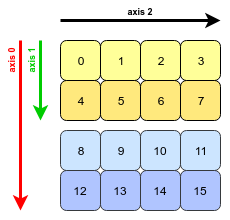
\includegraphics[width=\linewidth]{images/dml_strides_acces_matrix.png}
                \caption{Accès en ligne ou en colonne à une matrice.}
                \label{pic:dml_strides_acces_matrix}
                \end{subfigure}
            ~ %add desired spacing between images, e. g. ~, \quad, \qquad, \hfill etc. 
            %(or a blank line to force the subfigure onto a new line)
                \begin{subfigure}[b]{0.60\linewidth}
                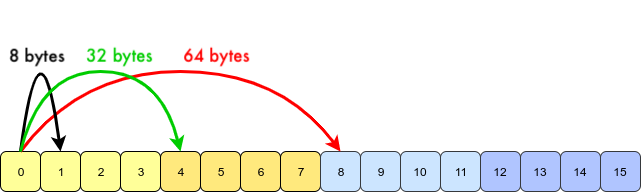
\includegraphics[width=\linewidth]{images/dml_strides_acces.png}
                \caption{Les accès en ligne ou en colonne impliquent des sauts en mémoire de différentes tailles.}
                \label{pic:dml_strides_acces}
                \end{subfigure}
            \caption{Exemple d'une application réalisant des accès en colonne à une matrice. Ces accès impliquent en réalité des sauts entre les adresses mémoires utilisées.}\label{pic:dml_strides_acces_main}
        \end{figure}
        % \subsubsection{Motivations}
    
    
        La grande majorité de ces applications ne réalisent pas suffisamment de calculs sur une donnée transférée pour masquer le temps de son accès mémoire. Ce déséquilibre de performance de l'architecture limite la performance de ces codes par celle du bus mémoire. 
        Pour ces applications, il est primordial que l'architecture soit capable d'anticiper le maximum des accès mémoire grâce à son matériel de préchargement mémoire (\textit{memory prefetcher}). Les pré-lecteurs mémoires sont conçus pour anticiper les accès avant qu'ils ne soient réalisés pour réduire la latence d'accès. Lorsque les accès sont simples (taille régulière, proches en mémoire), la majorité des architectures modernes obtiennent de très bonnes performances. Cependant, les accès par sauts peuvent être grands (supérieurs à plusieurs lignes de cache) et lorsque de multiples accès sont réalisés en concurrence, le pré-lecteur peut rencontrer des difficultés à les anticiper. 
    
        

    \subsubsection{Objectifs}
        
        Pour vérifier la bonne performance d'une architecture pour une application donnée, il n'est pas suffisant de vérifier que le bus mémoire est saturé. Pour l'illustrer, plusieurs expérimentations sont réalisées dans le \autoref{chap:methodo}. Ainsi, le benchmark \verb=DML_MEM= a été élaboré pour prouver l'efficacité du système mémoire pour les applications utilisant des motifs d'accès par \textit{strides}. 
    
        Le premier objectif du benchmark \verb=DML_MEM= est de caractériser la microarchitecture pour des applications utilisant des motifs d'accès par \textit{strides}. En mesurant ses performances, il est ensuite possible de prouver l’efficacité de l’utilisation du sous-système mémoire pour une application étudiée. 
        
        Le deuxième objectif est d'attirer l'attention du programmeur sur la complexité des architectures et de son impact sur les performances d'un code. En appréhendant cette complexité, il sera plus simple pour le programmeur d'apporter les bonnes modifications à son code pour tirer la pleine performance du bus mémoire.
        
        Une autre utilisation de notre outil peut aussi être réalisée par les concepteurs d'architectures qui veulent vérifier le bon fonctionnement du système mémoire pour ce type d'application. En effet, en utilisant ce benchmark nous avons trouvé certains dysfonctionnements majeurs dans un accélérateur prévu pour ce type d'applications. Grâce à notre outil, nous avons pu prouver que les performances théoriques de la plate-forme n'étaient pas accessibles par l'application. 
    
    
    \subsubsection{Comparaison avec l'existant}
    %%%%%%%%%%%%%%%%
        L'étude des différents benchmarks existants est réalisée dans la \autoref{sec:dev_existant}. Le seul outil s'approchant de notre démarche est le benchmark DISBench \cite{disbench}. Cependant, il ne bénéficie d'aucune méthode solide de vérification de la performance comme celui implémenté par \verb=DML_MEM=. De plus, il n'est en aucun cas prévu pour faciliter le test de multiples tailles de strides sur différentes tailles de jeux de données. Le code n'est plus maintenu depuis 6 ans et ne peut pas être exécuté sans erreur lors de l'exécution. Au moment de l'écriture de cette thèse, nous ne sommes au courant d'aucun outil permettant de remplir les objectifs fixés dans le section précédente. 


\subsection{Le benchmark DML\_MEM}
%%%%%%%%%%%%%%%%%%%%%%%%%%%%%%%%%%%%%%%%%%%%%%%%%%%%%%
    Le motif d'accès par \textit{stride} est donc très courant dans le calcul haute performance. La distance entre deux accès peut varier d'une application, ou d'un jeu de données, à l'autre. Pour caractériser les plateformes pour ces applications, il est donc nécessaire de posséder un benchmark paramétrable permettant de faire varier la taille du jeu de données et du saut. Cette section présente comment est conçu le benchmark \verb=DML_MEM= et comment il peut être utilisé. Grâce à de nombreuses options, différentes parties de la microarchitecture peuvent être testée: caches, TLB, bus mémoire.


    \subsubsection{Concept}
    %%%%%%%%%%%%%%%%
        
        Le principe du benchmark est d'accéder à un tableau en utilisant différentes tailles de strides. Pour chaque stride une mesure de performance est réalisée. Une fois toutes les tailles de stride mesurée, le benchmark augmente la taille du jeu de données utilisé (voir \autoref{pic:dml_stride_intro}). La vitesse d'évolution de la taille des strides et du jeu de données peut être paramétrée. Les accès peuvent être réalisés en lecture ou en lecture/écriture.
       
        \begin{figure}[h!]
        \center
        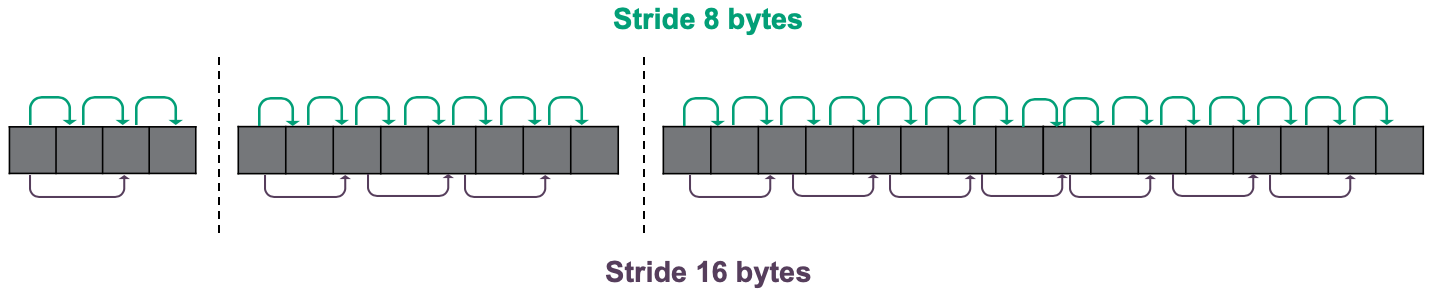
\includegraphics[width=14cm]{images/dml_stride_intro.png}
        \caption{\label{pic:dml_stride_intro}Évaluation de la performance de deux tailles de stride (8 et 16 bytes) sur trois jeux de données de tailles différentes.}
        \end{figure}

    
    \subsubsection{Développement}
    %%%%%%%%%%%%%%%%

        Le benchmark se déroule en deux étapes: la configuration et son exécution.
        Lors de la configuration, les différents paramètres nécessaires pour l'exécution du benchmark sont extraits de la ligne de commande ou utilisent, le cas échéant, des valeurs par défaut. Les différentes versions du benchmark (mode d'accès, taille du déroulement des boucles) sont toutes compilées, l'initialisation utilise un pointeur de fonction vers la bonne version requise par l'utilisateur. Ensuite, le jeu de données est initialisé (voir \autoref{sec:dml_init}). 
        La deuxième étape consiste à exécuter le benchmark et à mesurer ses performances. Pour une taille de jeu de donnée et une taille de stride, la bande passante effective maximale, minimale ou moyenne est mesurée et affichée. Pour cela, le benchmark mesure le temps nécessaire pour réaliser le noyau de calcul. Celui-ci, renvoie le nombre d'accès réalisés grâce à l'initialisation du tableau durant la première étape. 
            \begin{verbatim}
time1 = get_micros();
num_ops = p->m_BENCHMARK();
time2 = get_micros();
bande_passante = calcul_bw(num_ops, time2 - time1);
            \end{verbatim}
            
        Ces mesures sont affichées au fur et à mesure de l'avancée du benchmark ainsi que dans un fichier de \textit{log}. Ce fichier peut ensuite être utilisé par un script pour afficher l'évolution de la performance de chaque stride en fonction de la taille du jeu de donnée. 
            
\begin{verbatim}
>./dml --type read --cacheline 64 --matrixsize 10000 --stride 8,64,256
...
Stride  S   ->          8         64        256
Value       ->    AVERAGE    AVERAGE    AVERAGE
       7.0 KiB     117.46          -          -
      81.0 KiB     114.29      88.24      74.12
      76.3 MiB      80.87      13.41       8.61
       7.5 GiB      80.35      13.11       7.18
...
\end{verbatim}

  

    \subsubsection{Les options}
    %%%%%%%%%%%%%%%%
        Le benchmark \verb=DML_MEM= accepte de nombreuses options. Grâce à celles-ci différentes configurations peuvent être utilisées pour tester différents scénarios sur différentes parties de la microarchitecture. Nous décrivons ici les options les plus utiles pour l'utilisateur. Les nombreuses options peuvent être affichées avec l'option \verb|--help|.
        
        
        \paragraph{-{}-stride, -{}-minstride, -{}-maxstride, -{}-stridemode} Ces quatre premières options permettent de définir quelles sont les différentes strides à utiliser pour réaliser les mesures. La première d'entre elles, permet à l'utilisateur de choisir une ou plusieurs à réaliser. Pour cela, une liste de taille de strides séparées par des virgules doit être entrée. Les trois dernières options permettent de générer automatiquement des strides à utiliser dans un intervalle $[min, max]$. L'option \verb|--stridemode| peut être utilisée avec les valeurs \textit{even} et \textit{odd} pour décaler les strides ainsi générées. Cela permet d'éviter des strides utilisant seulement des multiples de deux, pouvant être affectées par certaines caractéristiques de la microarchitecture (taille ligne de cache, taille des caches...). 
        
        \paragraph{-{}-matrixsize, -{}-minlog, -{}-maxlog, -{}-steplog, -{}-log} Ces 5 options permettent de définir la taille des jeux de données à utiliser. Leur taille évolue plus ou moins rapidement en fonction de la valeur de \verb|--steplog| jusqu'à atteindre la taille \verb|max| ou bien celle de la matrice donnée avec l'option \verb|--matrixsize|. L'option \verb|--log| permet de donner la même valeur à \verb|min| et \verb|max| pour ne réaliser la mesure que sur une taille de jeux de données. S'il est utilisé avec la valeur $0$, le benchmark utilise la totalité du tableau. Couplées avec l'option \verb|--stride|, ces deux options permettent d'utiliser le benchmark pour n'accomplir qu'une seule mesure: un jeu de donnée, une stride.
        
        Ces 9 premières options sont les options principales du benchmark. Elles permettent de réaliser une multitude de mesures: performance des niveaux de caches, performance de la mémoire, fiabilité du pré-chargement, mesure de la taille d'une ligne de cache. Dans la \autoref{sec:dml_bad_stride} nous montrons comment ces options peuvent être utilisées pour identifier des tailles de strides ayant de mauvaises performances.
    
    
        \paragraph{-{}-type, -{}-unroll, -{}-mode} Ces trois options permettent de choisir le benchmark à utiliser. L'option \verb|--type| permet de réaliser les accès en lecture ou en lecture/écriture. La deuxième option permet d'appliquer l'optimisation du déroulement de boucle dont les différentes versions (déroulement de 2 à 64 fois) ont été programmées manuellement. La troisième option permet de choisir le mode d'accès. Par exemple l'utilisation de différents pointeurs pour réaliser plusieurs accès notamment lorsque l'option \verb|--unroll| est utilisée. L'analyse de la performance de ces options est réalisée dans la \autoref{sec:dml_unroll}.

        \paragraph{-{}-hugepages} Cette option permet d'allouer la mémoire pour le jeu de données en utilisant des pages de 2 MiB contre 4 KiB habituellement. La caractérisation des pages larges est réalisée dans la \autoref{sec:dml_large_page}.
        
        \paragraph{-{}-annotate} Cette option est utilisée lorsque l'activité du bus mémoire est mesurée avec l'outil YAMB (\autoref{sec:yamb}). Le benchmark ajoute une trace lors de chaque nouvelle stride utilisée et lorsque la taille du jeu de données change. Grâce à cette option, il est possible de corréler l'activité du bus avec une configuration particulière du benchmark. Cette option est utilisée dans la \autoref{sec:dml_cache_ok} pour mesurer l'activité du bus mémoire lorsqu'un jeu de donnée de la taille du dernier niveau de cache est utilisé. 

        \paragraph{Version parallèle} La dernière configuration du benchmark est la version parallèle utilisant MPI. Celle-ci doit être générée grâce à l'outil \textit{cmake} et la commande \verb|cmake -DOPT_BUILD_MPI=ON|. Grâce à cette version, plusieurs coeurs peuvent exécuter la même version du benchmark. Cette version du benchmark nous permet dans la \autoref{sec:dml_saturation} de mesurer l'évolution du débit mémoire lorsque des coeurs sont ajoutés.
        
    
    \subsubsection{Validation des résultats}
    %%%%%%%%%%%%%%%%

    Une grande difficulté lors de l'élaboration d'un benchmark est de s'assurer que la performance mesurée est bien celle du code attendu. En effet, le compilateur peut appliquer certaines optimisations pour accélérer l'application. Ensuite, l'architecture elle-même peut se rendre compte de l'artificialité du code et en court-circuiter une partie. Dans les deux cas, le problème est que la mesure de la performance ne rend pas compte de la réalité du code et de la mesure attendue par le programmeur. 
    
    Pour éviter ces deux pièges, le benchmark \verb=DML_MEM= initialise le jeu de données avec deux valeurs suivant le type de l'accès voulu (lecture ou lecture/écriture). Lorsque le benchmark utilise des accès en lecture, le jeu de données est initialisé avec la valeur \textbf{1}, car chaque lecture occasionne un transfert sur le bus mémoire. 
    Lorsque le benchmark utilise le mode de lecture/écriture, le jeu de données est initialisé avec la valeur \textbf{2}. Chaque ligne doit être lue puis réécrite occasionnant deux passages sur le bus mémoire. Pour chaque accès la valeur contenue dans le tableau est stockée dans une variable de compteur.  L'utilisation de chaque valeur pour l'ajouter au compteur empêche le compilateur et l'architecture d'appliquer certaines optimisations. À la fin de l'exécution, le benchmark retourne cette variable permettant de compter le nombre total d'accès effectivement réalisés.
    

    
    
    
    
    
    
    
    
\subsection{Résultats}
%%%%%%%%%%%%%%%%%%%%%%%%%%%%%%%%%%%%%%%%%%%%%%%%%%%%%%

    Dans cette section nous présentons les principaux résultats obtenus avec le benchmark DML\_MEM présenté précédemment. L'objectif est de montrer au lecteur les différentes mesures rendues possibles par l'utilisation de l'outil. Les tests sont principalement réalisés sur l'architecture des processeurs Intel Skylake. 


    \subsubsection{Choix du compilateur}
    %%%%%%%%%%%%%%%%
    
        Contrairement au benchmark du générateur de kernel (voir \autoref{sec:kg}), le code de DML\_MEM n'est pas écrit directement en assembleur. La qualité du compilateur peut donc avoir un impact significatif sur ses performances. Avant de réaliser plus d'expérimentations, nous avons testé deux compilateurs (GCC 8.2 et ICC 19.0) avec différents drapeaux de compilation. Avec d'anciennes versions de GCC (telle que la version 4.8), nous avons mesuré une amélioration d'un facteur deux en utilisant les drapeaux \verb|-O3 -march=skylake-avx512|. Le compilateur ayant reçu de nombreuses améliorations depuis, nous n'avons trouvé aucun drapeau permettant d'améliorer les performances de ce dernier. Nous l'avons comparé avec la version 19.0 du compilateur d'Intel ICC couplé avec le drapeau \verb|-O3|. Les performances mesurées dans les différents niveaux de la hiérarchie mémoire sont présentées dans le \autoref{tab:dml_compiler}.

        \begin{table}[h!]
        \centering
        \begin{tabular}{|l|c|c|}
        \hline
        Perf. GB/s & GCC 8.2 & ICC 19.0 \\ \hline
        L1 & 58 & 310 \\ \hline
        L2 & 56 & 161 \\ \hline
        L3 & 26 & 26 \\ \hline
        Memory & 12.5 & 12.5 \\ \hline
        \end{tabular}%
        \caption{Performance du benchmark DML\_MEM compilé avec les compilateurs GCC et ICC mesurée en GB/s. Le drapeau d'optimisation \text{-O3} est utilisé dans les deux cas.}
        \label{tab:dml_compiler}
        \end{table}

        Lorsque le jeu de données tient dans le premier niveau de cache, nous avons mesuré des différences de performances du benchmark pouvant aller jusqu'à un facteur 8. Cet écart de performance entre les deux compilateurs se réduit lorsque la taille du jeu de données augmente. En effet, la performance du bus mémoire pour les deux compilateurs est équivalente. Nous expliquons cet écart de performance dans les premiers niveaux de cache par la mauvaise performance du code généré par le compilateur GCC. Le premier niveau de cache des processeurs Skylake est capable de fournir 128 octets par cycle, soit une bande passante de 345 GB/s. Le code généré par GCC ne parvient pas à utiliser plus de 58 GB/s. Nous avons mesuré que le benchmark compilé par GCC utilisé deux fois plus d'instructions que celui compilé par ICC. Le benchmark GCC n'est alors pas \textit{memory bound} mais \textit{compute bound}. La bande passante disponible se réduisant lorsqu'on remonte dans la hiérarchie mémoire, l'impact de la qualité du code est aussi réduit. Les performances du benchmark compilé par ICC étant toujours supérieures à celles produites par GCC, nous utiliserons le compilateur d'Intel dans les prochaines expérimentations. Lorsque de nouvelles versions sont disponibles ou que d'autres architectures sont étudiées, nous conseillons de toujours tester les différentes versions de compilateurs avec les drapeaux de compilation adéquats.
    
    
    
    \subsubsection{Mesurer la taille d'une ligne de cache}
    %%%%%%%%%%%%%%%%
        Connaître la taille d'une ligne de cache de l'architecture est nécessaire pour obtenir les mesures correctes par le benchmark. Cette taille peut aussi être nécessaire lors du développement d'une application pour disposer les données de façon optimale. Nous montrons dans cette expérimentation comme celle-ci peut être retrouvée en utilisant le benchmark DML\_MEM. Pour cela, nous désactivons le \textit{memory prefetch} pour l'empêcher d'anticiper le chargement d'une ou plusieurs lignes de cache avant son accès. Le jeu de données utilisé doit quand à lui plus grand que le dernier niveau de cache. La taille des lignes de cache des architectures modernes est généralement comprise entre 32 et 256 bytes. Nous utilisons le benchmark pour mesurer la performance du système mémoire en utilisant des strides de puissance de 2 allant de 8 à 256 bytes. Les performances ainsi mesurées sont présentées dans le \autoref{tab:dml_cache_line}.
    
        \begin{table}[]
        \centering
        \begin{tabular}{|l|c|c|c|c|c|c|}
        \hline
        Taille de la stride (byte) & 8 & 16 & 32 & 64 & 128 & 256 \\ \hline
        Bande passante (GB/s) & 31.58 & 25.84 & 14.50 & 7.62 & 7.65 & 7.62 \\ \hline
        \end{tabular}%
        \caption{Pour un jeu de données de 1 GiB, mesure de la performance de plusieurs tailles de stride lorsque le pré-chargement mémoire est désactivé.}
        \label{tab:dml_cache_line}
        \end{table}
        
         L'interprétation de ces résultats doit être la suivante. Pour des strides de 64, 128 ou 256 bytes, la performance est la même. Il est important de rappeler que le benchmark mesure le débit mémoire atteint par l'application et non le trafic mémoire du bus. Ceci indique que pour ces trois cas, le processeur attend une ligne de cache pour réaliser un accès. Le prochain accès étant situé sur une autre ligne de cache, leur performance est équivalente. Lorsqu'une stride de 32 bytes est utilisée, la performance double, indiquant que la taille d'une ligne de cache est de 64 bytes. En effet, le processeur est capable de réaliser deux fois plus d'accès. Ceci est possible, car lorsqu'un premier accès est réalisé sur une ligne de cache, le suivant le sera aussi. La donnée est alors déjà présente dans le cache L1. L'utilisation d'une stride de 16 bytes améliore encore la performance du benchmark sans doubler pour autant. En effet, comme dans la première expérimentation le code devient \textit{compute bound}. Le benchmark additionne des nombres flottants et la performance du code est alors limitée par l'ALU. 
    
    
    \subsubsection{Performances de différentes tailles de strides} \label{sec:dml_bad_stride}
    %%%%%%%%%%%%%%%%
        
        Un objectif principal de notre benchmark est de vérifier le bon comportement du processeur lors d'accès mémoire utilisant des sauts mémoires constants. Pour cela, nous avons développé un script qui permet d'exécuter le benchmark avec un grand nombre de strides et d'afficher leur performance dans un graphique. La \autoref{pic:dml_strides_bad} montre le résultat d'une telle exécution. Pour chaque stride et chaque taille de jeu de données, une mesure est réalisée. Pour faciliter la lecture du graphique, nous avons coloré les strides en fonction de leur taille en allant du bleu (pour les strides les plus petites) au rouge (pour les plus grandes). Nous remarquons que les strides de grande taille (plusieurs MiB) ont de meilleures performances que celle de petite taille. En effet, même pour des tailles de jeu de données de plusieurs centaines de mégaoctets (ne pouvant pas tenir dans le cache), le benchmark mesure des performances similaires à si le jeu de données se trouvait dans le cache. En réalité, pour des grandes tailles de strides, le jeu de données réellement utilisé par le benchmark peut être contenu dans les différents niveaux de cache. 
      
        \begin{figure}
        \center
        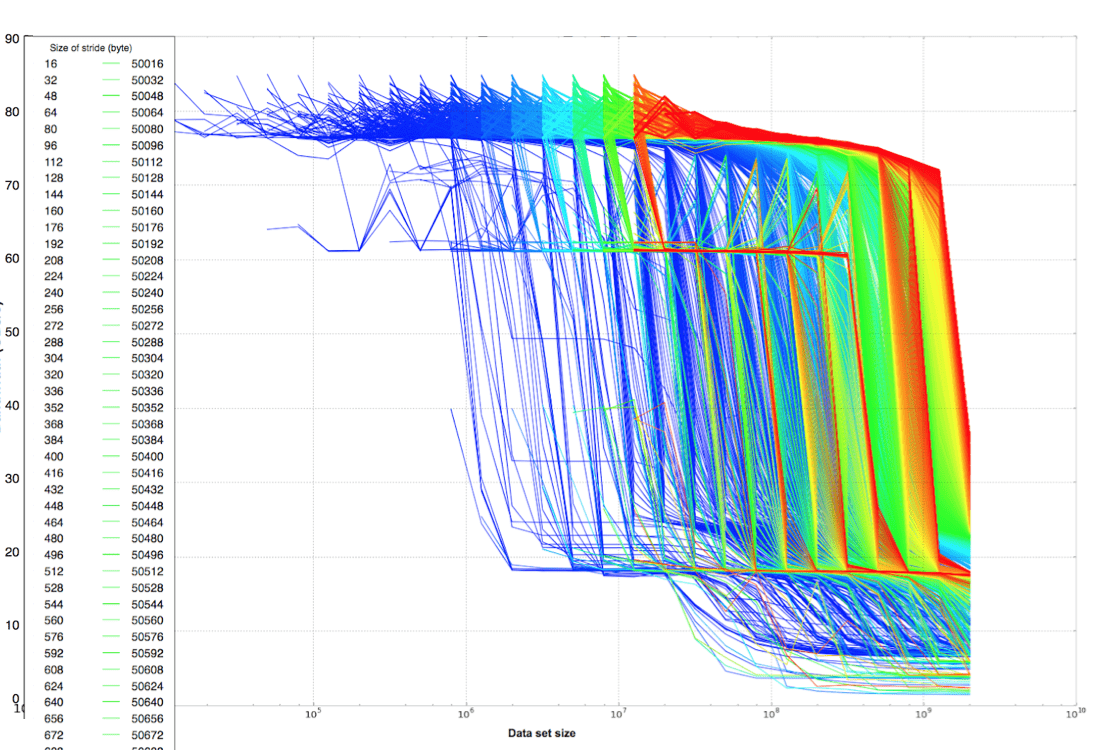
\includegraphics[width=12cm]{images/dml_strides_bad.png}
        \caption{\label{pic:dml_strides_bad} Performance du benchmark pour différentes tailles de strides (couleurs).  }
        \end{figure}
        
        Nous remarquons sur la \autoref{pic:dml_strides_bad} que certaines strides ont des comportements différents que des strides de tailles proches (donc de couleurs proches aussi). En effet, des groupes de strides ont des performances bien plus faibles que d'autres et les mêmes résultats sont obtenus en utilisant des pages larges pour réduire l'impact sur la TLB. Nous avons isolé certaines d'entre elles et reporté leur performance dans le  \autoref{tab:dml_bad_strides}. Pour réaliser ces mesures, la commande suivante a été utilisée: 
        \begin{verbatim}
./dml --steplog 0.01 --unroll 8 --mode special --type read --cacheline 64 
      --stride 73704,73728,77816,77824,81928,81920 --measure 10 --matrixsize 10000
        \end{verbatim}
        
        
        \begin{table}[]
        \centering
        \begin{tabular}{|c|c|c|c|c|}
        \hline
        \rowcolor[HTML]{EFEFEF} 
        Taille de la stride (byte) & Bande passante (GB/s) & Nb. inst. & IPC & LLC Miss \\ \hline
        \rowcolor[HTML]{FFFFC7} 
        73704 & 24.54 & 690071400 & 0.34 & 21100474 \\ \hline
        \rowcolor[HTML]{FFFFC7} 
        73728 & 2.04 & 690064918 & 0.22 & 30612018 \\ \hline
        \rowcolor[HTML]{E8FFFE} 
        77816 & 24.53 & 688909428 & 0.33 & 21152403 \\ \hline
        \rowcolor[HTML]{E8FFFE} 
        77824 & 4.01 & 688905576 & 0.27 & 30144907 \\ \hline
        \rowcolor[HTML]{E6FFE6} 
        81928 & 24.76 & 690692156 & 0.33 & 21194483 \\ \hline
        \rowcolor[HTML]{E6FFE6} 
        81920 & 4.03 & 690693382 & 0.27 & 30794354 \\ \hline
        \end{tabular}%
        \caption{Différence de performance de trois couples de stride}
        \label{tab:dml_bad_strides}
        \end{table}
        
        
        Le benchmark qui utilise une \textit{mauvaise} stride est \textit{latency bound}. En effet, nous avons réalisé différentes mesures telles que le nombre de \textit{miss} du dernier niveau de cache ou l'activité du bus mémoire. On remarque que l'IPC est plus faible et que le nombre de \textit{miss} est lui plus élevé pour ces strides. L'analyse de l'activité du bus mémoire montre qu'il est loin d'être saturé. Si la ligne de cache n'est pas présente dans un des niveaux de cache, et que le bus n'est pas saturé, c'est que le processeur l'attend et n'a pas anticipé son manque (\textit{miss}). La question est alors de savoir pourquoi pour une certaine taille la ligne de cache est présente dans le cache et que pour une stride plus grande de quelques bytes elle n'y soit pas. L'explication vient de la taille des strides utilisées. Nous avons utilisé des strides de taille $ Stride_{n+1} = Stride_n + 16 bits$ avec $Stride_0 = 16 bytes$. En utilisant des tailles de multiple de 16 certaines d'entre elles génèrent des conflits avec la politique de remplacement de lignes de caches. Ainsi, certaines d'entre elles mettent la pression seulement sur une partie du cache, le rendant inefficace. Le processeur doit donc attendre pour une majorité des accès que la ligne de cache soit transféré depuis la mémoire rendant le code \textit{latency bound}.
        
        Nous avons ensuite réalisé la même expérimentation en décalant la taille des strides utilisées en commençant avec une stride minimale $Stride_0 =  8 bytes$. Ainsi, aucune stride utilisée n'est multiple de 32, et aucune d'entre elle obtient de performance inattendue (voir \autoref{pic:dml_strides_good}).
        
        
        \begin{figure}
        \center
        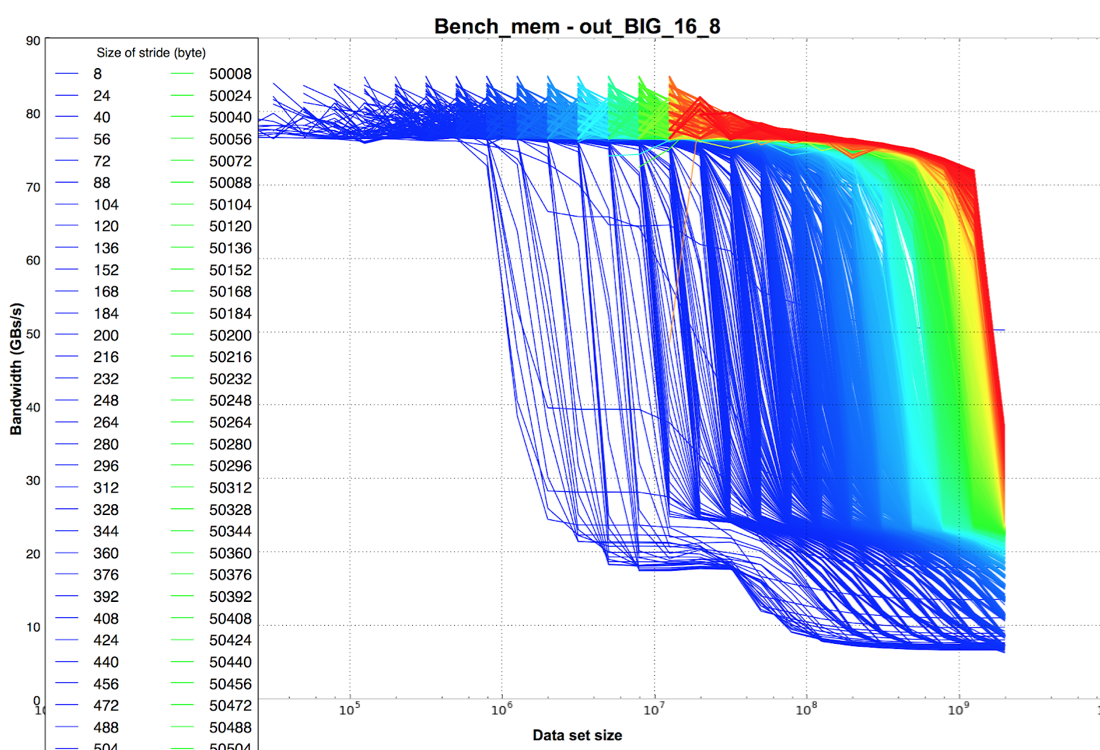
\includegraphics[width=12cm]{images/dml_strides.png}
        \caption{\label{pic:dml_strides_good} Performance du benchmark pour différentes tailles de strides (couleurs).  }
        \end{figure}
        
        À travers cette expérimentation, nous avons voulu montrer qu'un code aussi simple qu'il est peut avoir des performances inattendues. La complexité des architectures modernes est telle qu'elle peut avoir une incidence forte sur la performance des applications. Pour des strides aussi longues (plusieurs MiB), le \textit{memory prefetcher} ne semble pas arriver à anticiper ces accès. Si une application réalise ce type d'accès, le programmeur doit s'assurer de ne pas réaliser des strides de cette taille en ajoutant du \textit{padding} (remplissage) pour décaler artificiellement les données accédées. Une autre optimisation lors d'accès à certains champs d'objets contenus dans un tableau est de regrouper ces mêmes champs dans une structure spécifique. Ainsi, ces champs sont contigus en mémoire. 
        
        
        

    \subsubsection{Saturation du bus mémoire}\label{sec:dml_saturation}
    %%%%%%%%%%%%%%%%
        Que ce soit pour notre modèle de performance ou d'autres de type \textit{Roofline}, il est nécessaire de connaître la bande passante maximale atteignable par un processeur. Pour cela, nous avons exécuté le benchmark en utilisant différents nombres de coeurs. Les résultats sont visibles sur le graphique de la \autoref{pic:dml_bw_mpi}. Sur ce processeur, notre benchmark arrive à obtenir une bande passante mémoire maximale de 114 GB/s. La loi de Little ne permet pas à un seul coeur de saturer la totalité du bus mémoire. Nous montrons à travers cette expérimentation qu'il faut au moins 15 coeurs pour le saturer. Les coeurs supplémentaires ne permettent pas ensuite d'améliorer le débit mémoire, car le bus est saturé. Pour des codes \textit{memory bound} il peut alors être intéressant d'en désactiver certains ou de ne pas investir dans des processeurs avec plus de coeurs. Nous présentons dans la \autoref{sec:dml_core_vs_freq} un script permettant de réaliser cette recherche du nombre minimal de coeurs permettant de saturer le bus mémoire. 
        
        \textit{TODO: comparaison avec STREAM}
        
        \begin{figure}
        \center
        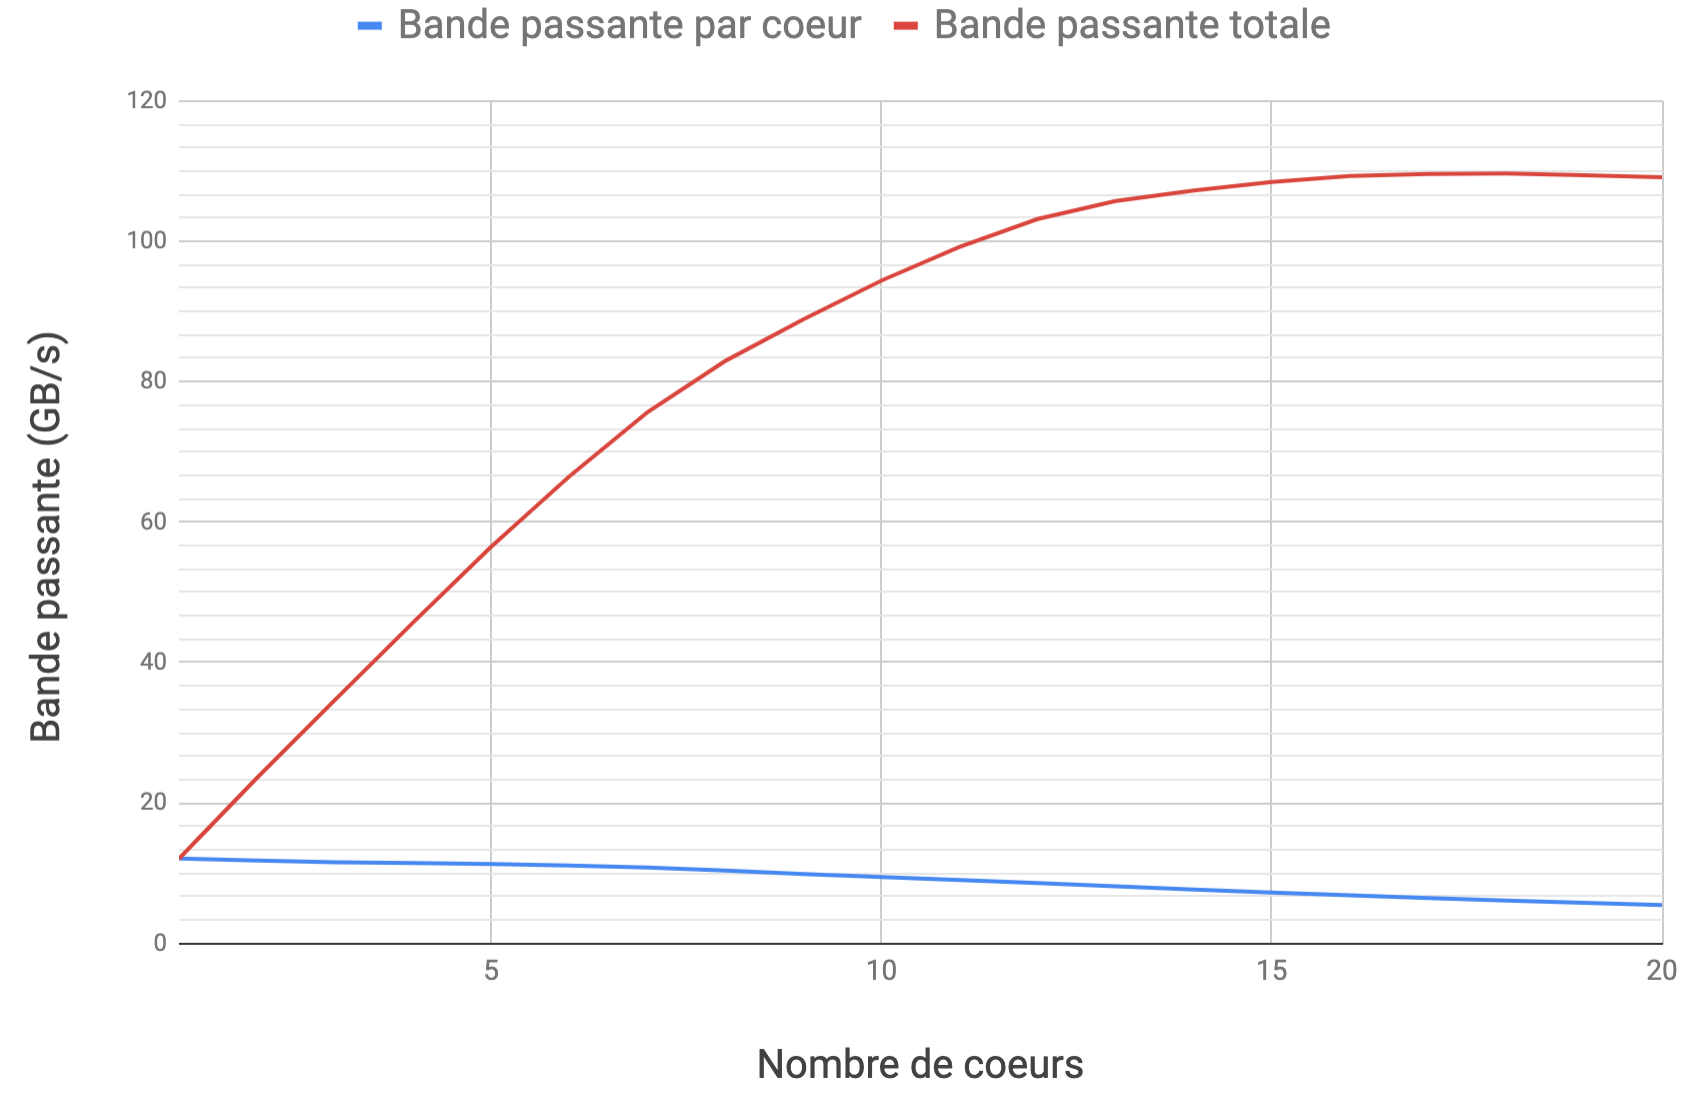
\includegraphics[width=10cm]{images/dml_bw_mpi.png}
        \caption{\label{pic:dml_bw_mpi} Bande passante mémoire atteinte pour différent nombre de coeurs}
        \end{figure}
        
    
    
    

    \subsubsection{Vérifier le bon fonctionnement des caches} \label{sec:dml_cache_ok}
    %%%%%%%%%%%%%%%%
        Les caches des architectures modernes se sont complexifiées et sont devenues très efficaces pour accélérer les accès mémoires. Cependant, sur des architectures différentes que celles utilisées communément, il peut être intéressant de vérifier leur bon fonctionnement. Nous montrons dans cette expérimentation les tests pouvant être réalisés.
        
        La première vérification est de s'assurer de l'indépendant des caches propres à chaque coeur. Dans le cas des processeurs Skylake, les deux premiers niveaux sont privés à chaque coeur. Nous avons implémenté une option pour annoter la taille de niveau de cache sur le graphique final. Les résultats de deux exécutions sur 1 et 20 coeurs sont présentés sur la \autoref{pic:dml_cache}. La performance lorsque le jeu de donnée est contenu dans le cache L1 et L2 n'est pas impacté par l'utilisation d'autres coeurs. Les performances se dégradent lorsque le jeu de données commence à remplir le dernier niveau de cache, commun à tous les coeurs. La même expérimentation peut être menée sur les différents caches L3 de plusieurs processeurs d'un même serveur.
        
        \begin{figure}
        \centering
            \begin{subfigure}[b]{0.47\linewidth}
            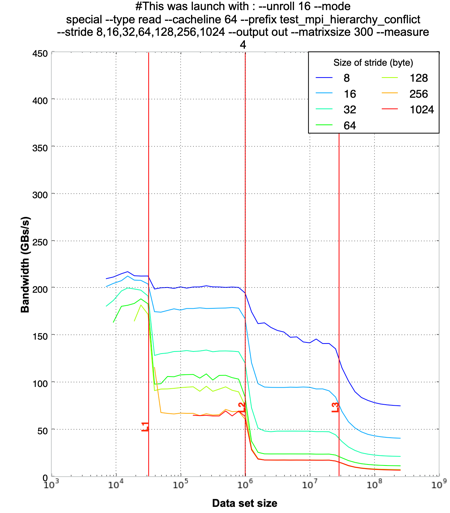
\includegraphics[width=\linewidth]{images/dml_cache_1core.png}
            \caption{1/20 coeur actif}
            \label{pic:dml_cache_1core}
            \end{subfigure}
        ~ %add desired spacing between images, e. g. ~, \quad, \qquad, \hfill etc. 
        %(or a blank line to force the subfigure onto a new line)
            \begin{subfigure}[b]{0.47\linewidth}
            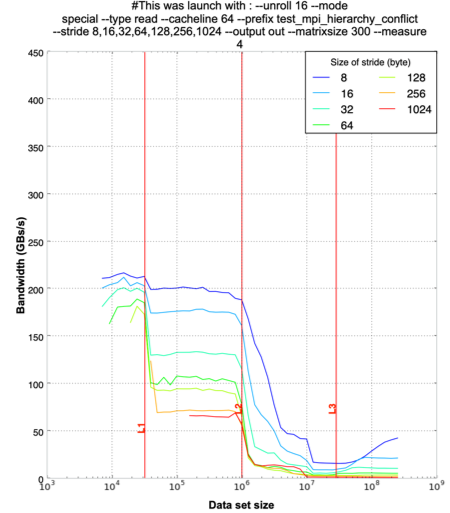
\includegraphics[width=\linewidth]{images/dml_cache_20core.png}
            \caption{20/20 coeurs actifs}
            \label{pic:dml_cache_20core}
            \end{subfigure}
        \caption{Performance du benchmark lorsqu'un ou la totalité des coeurs sont actifs. Les résultats montrent que les cache L1 et L2 ne sont pas affectés par l'utilisation d'autres coeurs.}\label{pic:dml_cache}
        \end{figure}
        
        Une deuxième expérimentation pouvant être menée au niveau des caches est la vérification du fonctionnement du cache L3. Pour cela, nous utilisons un jeu de donnée dont la taille évolue jusqu'à remplir le dernier niveau de cache.  En parallèle, nous mesurons l'activité sur le bus mémoire avec l'outil YAMB (voir \autoref{pic:dml_L3_sharing}). Cette expérimentation peut être réalisée avec les commandes suivantes:
        \begin{verbatim}
./monitoring_bw_main.sh --start
./dml --steplog 0.01 --unroll 2 --type read --cacheline 64 --stride 64  
      --matrixsize 100 --measure 1000 --minlog 6.1 --annotate log_mem.annotate
./monitoring_bw_main.sh --stop
        \end{verbatim}
        
         \begin{figure}
        \center
        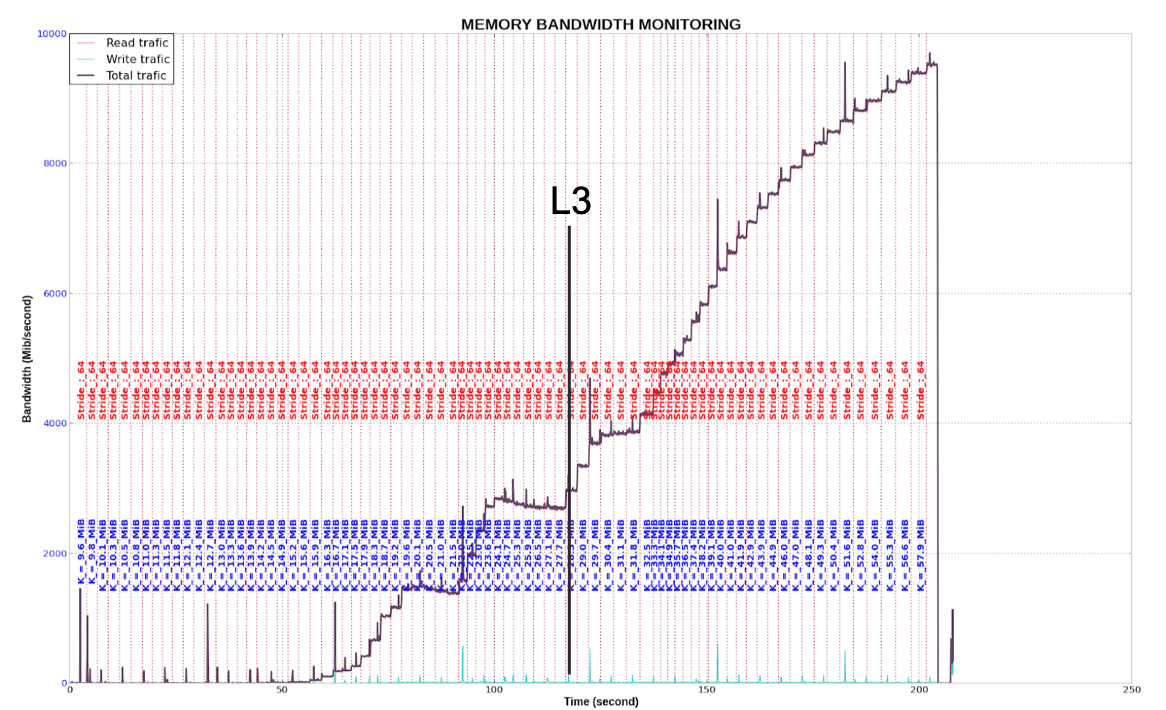
\includegraphics[width=14cm]{images/dml_L3_sharing.png}
        \caption{\label{pic:dml_L3_sharing} Évolution de l'activité du bus mémoire en fonction de la taille du jeu de donnée.}
        \end{figure}
        
        Nous montrons ainsi que pour un cache L3 de 28 MiB ne parvient pas à garder la totalité d'un jeu de donnée dépassant les 16 MiB. Au-delà de cette taille, YAMB mesure de l'activité sur le bus mémoire pouvant atteindre les 3 GB/s pour un jeu de donnée de la taille du L3 (28MiB). 
        
        
        Cette mauvaise utilisation du cache peut être due au phénomène de coloration de page discuté dans les expérimentations suivantes. Cette caractéristique impacte la performance de chaque coeur, car certaines données sont éjectées du cache et génèrent un évènement de \textit{miss}. Nous avons réalisé une seconde expérimentation en utilisant deux jeux de données de 20 et 28 Mib. Pour chaque jeu, nous utilisons progressivement la totalité des coeurs. Le résultat présenté sur la \autoref{pic:dml_bw_cacheL3} montre que le phénomène de \textit{trash} est encore plus fort lorsque plusieurs coeurs sont utilisés. Le trafic généré atteint les 19 GB/s pour 6 coeurs se partageant un jeu de données de 28 MiB. Cependant, la performance entre les deux benchmarks est identique, permettant de conclure du bon fonctionnement du préchargement mémoire. Si une architecture ne possède pas un composant aussi efficace, il peut alors être intéressant de réduire la taille des jeux de données utilisés. Pour certaines optimisations, tel que le \textit{cache blocking}, nos expérimentations nous ont montrés que d’utiliser 80\% de la capacité du dernier niveau de cache était le plus efficace.
        
        \begin{figure}
        \center
        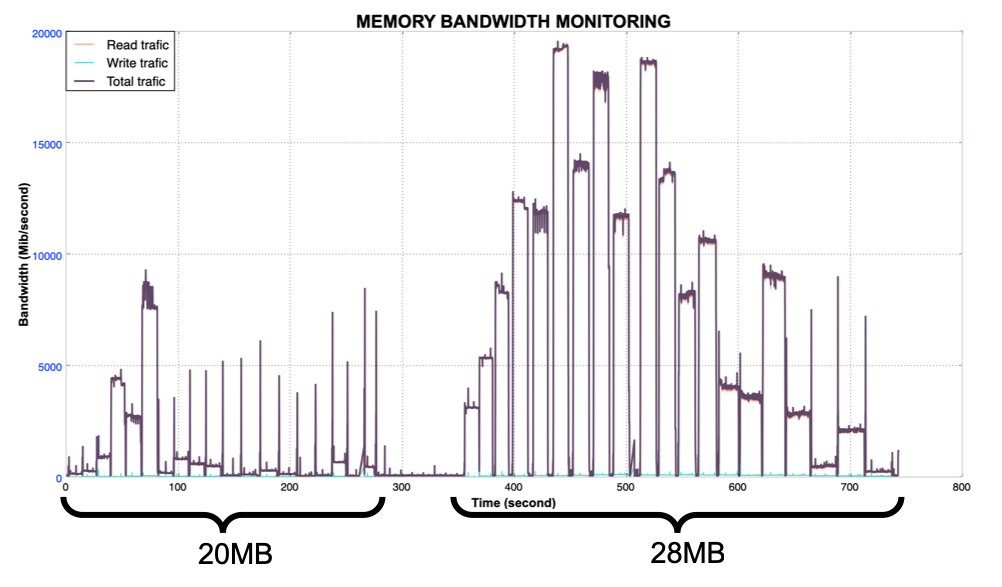
\includegraphics[width=14cm]{images/dml_bw_cacheL3.png}
        \caption{\label{pic:dml_bw_cacheL3} Évolution du trafic mémoire pour deux jeux de données de 20 et 28 MiB. Chaque jeu est accédé par 1 à 20 coeurs.}
        \end{figure}
        
        

    \subsubsection{Préchargement mémoire}
    %%%%%%%%%%%%%%%%
        
        Dans l'expérimentation précédente nous montrons que le préchargement mémoire permet de maintenir la bonne performance du benchmark même lorsque des données sont évincées du cache. Dans cette partie nous questionnons l'utilité de son activation permanente. 
        
        Le benchmark \verb=DML_MEM= a été utilisé pour réaliser des accès à un jeu de donnée dépassant la taille du plus grand niveau de cache. La \autoref{pic:dml_prefetch} montre la bande passante mémoire atteignable par un seul coeur lorsque le pré-chargement est activé ou non. On remarque que les performances sont similaires sauf pour une \textit{stride} de 64 bytes, correspondant à la taille d'une ligne de cache. Pour une telle \textit{stride}, la bande passante mémoire atteinte est réduite de 40\% lorsque le pré-chargement est désactivé.
        La raison de cette baisse vient d'un mécanisme couramment utilisé dans les architectures appelé le pré-chargement adjacent. Lors d'un accès mémoire, celui-ci anticipe les futurs accès en chargeant aussi la ligne de cache suivante. Les codes parcourent souvent la mémoire de façon contiguë (données d'un tableau, instruction d'un programme). Avec l'utilisation d'une \textit{stride} de 128 bytes, nous montrons que le mécanisme de pré-chargement n'améliore plus les performances, car il ne s'occupe de charger que la ligne de caches adjacente (inutilisée). En désactivant le pré-chargement adjacent, les performances sont même supérieures, car le bus mémoire n'est pas affecté par le transport de lignes de cache inutiles.
        
        \begin{figure}
        \center
        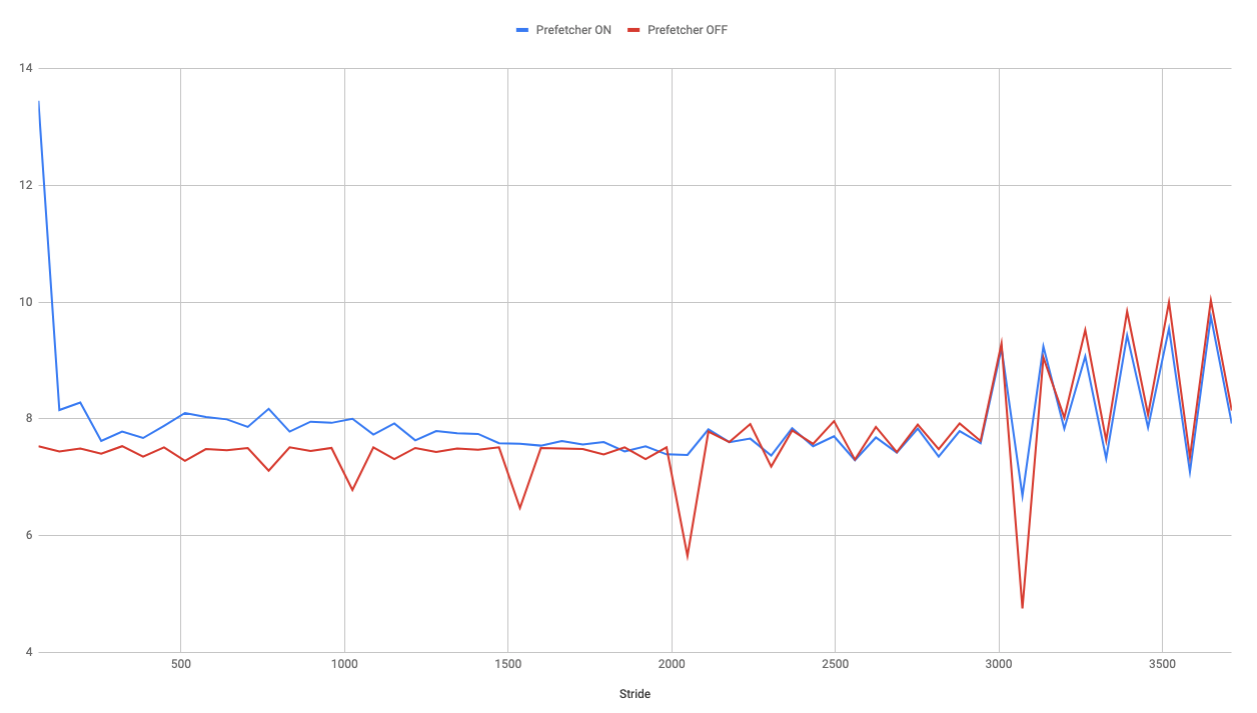
\includegraphics[width=10cm]{images/dml_prefetch.png}
        \caption{\label{pic:dml_prefetch} Performance mémoire d'un coeur lors de l'activation ou non du pré-chargement mémoire. }
        \end{figure}
         
        Pour montrer que l'activation du pré-chargement peut altérer les performances d'une application, la version parallèle du benchamrk \verb=DML_MEM= a été utilisée. En effet, le pré-chargement de la ligne de cache adjacente n'est bénéfique que si elle est ensuite utilisée. Lorsqu'un seul coeur est actif, le chargement de cette ligne de cache n'impacte pas la performance du benchmark, car le bus est loin d'être saturé (voir \autoref{pic:dml_prefetch}). La version parallèle de \verb=DML_MEM= peut être utilisé pour charger la totalité des coeurs du processeur pour réaliser un accès mémoires toutes les deux lignes de cache (\textit{stride} 128 bytes). La désactivation du pré-chargement permet d'atteindre des performances 16\% supérieures (91 GB/s contre 73 GB/s lorsque le pré-chargement est actif). Ce type d'accès plus grand que deux lignes de cache est très courant dans les applications. Il peut donc être avantageux de le désactiver le pré-chargement de la ligne de cache adjacente pour ces portions de codes. De plus, le pré-chargement de données peut être réalisé manuellement grâce à des instructions telle que \verb| __builtin_prefetch (&a[i+j]); |.

        Si une architecture possède un préchargement mémoire défaillant, il peut être intéressant de vérifier si les coeurs du processeur sont capables de générer suffisamment de requêtes mémoires pour saturer le bus. En utilisant la version \textit{MPI} du benchmark, nous avons mesuré la performance du benchmark avec le mécanisme de pré-chargement adjacent actif ou non, avec différent nombre de coeurs. La \autoref{pic:dml_prefetch_mpi} montre que si le pré-chargement adjacent est désactivé la totalité des coeurs ne suffisent pas à saturer le bus mémoire. 
        
        
        \begin{figure}
        \center
        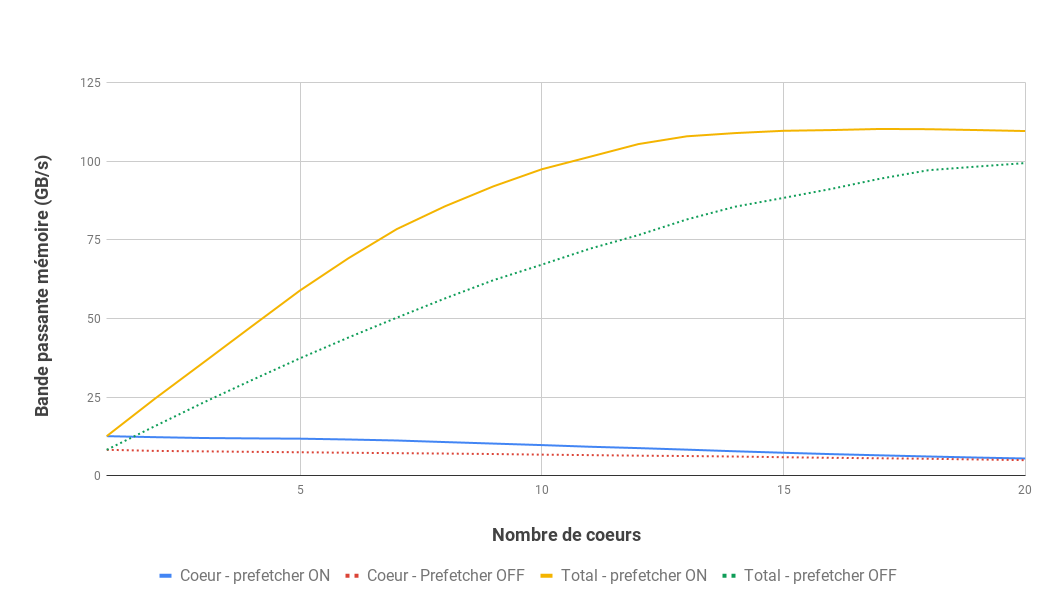
\includegraphics[width=14cm]{images/dml_prefetch_mpi.png}
        \caption{\label{pic:dml_prefetch_mpi} Performance du benchmark pour un jeu de données de 300 MiB avec un et plusieurs coeurs actifs lorsque le pré-chargement adjacent activé ou non.}
        \end{figure}
        
        
        
    
    \subsubsection{Déroulement de boucle} \label{sec:dml_unroll}
    %%%%%%%%%%%%%%%%
    Pour améliorer les performances du benchmark \verb=DML_MEM=, l'optimisation du déroulement de boucle à été utilisée. Au vu de l'amélioration des performances obtenues, cette section présente comment l'optimisation est implémentée et comment les applications peuvent en tirer partie. 
    Le déroulement de boucle est une optimisation permettant de réduire l'impact de code permettant le contrôle de la boucle (test, incrémentation). Le principe est de développer manuellement le code de plusieurs itérations dans la boucle et d'incrémenter ensuite la boucle de même nombre de déroulements. Ainsi, la proportion de code responsable du contrôle de la boucle est réduite par rapport à l'intérieur de la boucle. Une première version du code utilisé pour réaliser le déroulement est présentée dans l'\autoref{lst:dml_unroll_orig}. Pour permettre au processeur commencer les accès mémoire grâce au mécanisme d'exécution dans le désordre, 4 pointeurs différents sont utilisés. Chaque pointeur pointe vers une stride et la valeur est sommée dans la variable \verb|sum|. Les résultats obtenus par cette première version sont mauvais, notamment pour des jeux de données situés dans les premiers niveaux de cache (baisse de la performance d'un facteur trois). Cet effondrement de performance vient de l'incapacité du compilateur à appliquer sa propre optimisation de déroulement de boucle. Cette première version étant plus mauvaise, la performance est fortement dégradée. Par ce premier résultat, nous souhaitons attirer l'attention du programmeur sur le fait que le compilateur réalise déjà certaines optimisations. Il peut être contre-productif de la réaliser, soit même. 
    
    \begin{lstlisting}[label=lst:dml_unroll_orig ,language=C, caption=Première version du déroulement de la boucle par 4.]
for (rep = 0; rep < repeat; rep++) {
    DML_DATA_TYPE *p1 = mat;
    DML_DATA_TYPE *p2 = p1 + step;
    DML_DATA_TYPE *p3 = p2 + step;
    DML_DATA_TYPE *p4 = p3 + step;
    for (steps = 0; steps < ops_per_scan; steps++) {
        sum += *p1;
        p1 += xstep;
        sum += *p2;
        p2 += xstep;
        sum += *p3;
        p3 += xstep;
        sum += *p4;
        p4 += xstep;
    }
}
\end{lstlisting}


    L'erreur dans la première version du déroulement est l'utilisation d'une unique variable de sommation. En effet, cette unique variable qui doit être incrémentée à chaque lecture d'une stride crée une dépendance empêchant le code d'exécuter deux opérations d'addition par cycle. L'\autoref{lst:dml_unroll_spe} présente la version \textit{special} de l'optimisation du déroulement qui utilise autant de variables de sommation que de déroulements réalisés. Avec cette version, la performance du benchmark dans les caches L1 et L2 est améliorée respectivement de 12\% et 30\%. 
    
    \begin{lstlisting}[label=lst:dml_unroll_spe ,language=C, caption=Deuxième version du déroulement par 4 utilisant 4 variables sum.]
for (rep = 0; rep < repeat; rep++) {
    BM_DATA_TYPE *p1 = mat;
    BM_DATA_TYPE *p2 = p1 + step;
    BM_DATA_TYPE *p3 = p2 + step;
    BM_DATA_TYPE *p4 = p3 + step;
    for (steps = 0; steps < ops_per_scan; steps++) {
        sum1 += *p1;
        p1 += xstep;
        sum2 += *p2;
        p2 += xstep;
        sum3 += *p3;
        p3 += xstep;
        sum4 += *p4;
        p4 += xstep;
    }
}
return sum1 + sum2 + sum3 + sum4;
\end{lstlisting}
    
    La suite de cette expérimentation s'intéresse au nombre de déroulements de la boucle et de son impact sur la performance de benchmark. Pour cela, le benchmark a été exécuté en utilisant entre 1 et 64 déroulements sur un jeu de données remplissant 80\% du cache de niveau 2. Les résultats obtenus sont présentés dans le \autoref{tab:dml_unroll_bench}. Nous vérifions que l'optimisation du déroulement est bénéfique pour la performance du benchmark améliorant les performances progressivement de 117.8 GB/s à 337 GB/s pour un déroulement de boucle allant de 2 à 8 fois. On remarque que moins d'instructions sont exécutées et que le nombre d'instructions exécutées chaque cycle augmente de 2 à 3.22. Au-delà de 8 déroulements, la performance du benchmark se dégrade progressivement. Avec 64 déroulements de la boucle, le nombre d'instructions exécutées double et les performances s'effondrent à 140 GB/s. De nouveau, nous montrons ici que la mesure du nombre d'instructions exécuter chaque cycle n'est pas un bon indicateur pour évaluer la performance d'un code. 
    

    \begin{table}[h!]
    \centering
    \begin{tabular}{|c|c|c|c|}
    \hline
    \rowcolor[HTML]{EFEFEF} 
    \multicolumn{1}{|l|}{\cellcolor[HTML]{EFEFEF}Nb. de déroulements} & \multicolumn{1}{l|}{\cellcolor[HTML]{EFEFEF}Bande passante (GB/s)} & \multicolumn{1}{l|}{\cellcolor[HTML]{EFEFEF}Nb. d'instructions exécutée} & \multicolumn{1}{l|}{\cellcolor[HTML]{EFEFEF}Instruction par cycle} \\ \hline
    1 & 117.8 & 4204612342 & 2 \\ \hline
    2 & 235.47 & 3159994082 & 2.99 \\ \hline
    4 & 311.07 & 2634059908 & 3.28 \\ \hline
    8 & 337.96 & 2380891060 & 3.22 \\ \hline
    16 & 306.66 & 2483260088 & 3.07 \\ \hline
    32 & 315.17 & 2513084995 & 3.19 \\ \hline
    64 & 140.98 & 4993000253 & 2.87 \\ \hline
    \end{tabular}%
    \caption{Performance du benchmark \texttt{DML\_MEM} utilisant plusieurs taille de déroulement de la boucle pour un jeu de donnée atteignant 80\% du cache L2.}
    \label{tab:dml_unroll_bench}
    \end{table}
    
    Pour comprendre la mauvaise performance du code lorsqu'il est déroulé plus de 8 fois, nous avons extrait leur code assembleur. L'\autoref{lst:unroll4} montre comment le code du benchmark est généré lorsque 4 déroulements sont réalisés. On remarque que les 4 opérations d'additions sont vectorisées et qu'elles se suivent dans le code permettant à l'exécution dans le désordre de les exécuter deux par deux. On remarque aussi que 16 des 32 registres \verb|%xmm| sont utilisés. L'\autoref{lst:unroll16} expose le code assembleur du benchmark déroulant 16 fois la boucle. Le processeur utilise alors la totalité des 32 registres \verb|%xmm|. Cependant, ce n'est pas suffisant pour réaliser tous les traitements et il est obligé de stocker et charger certains éléments depuis la pile. L'exécution des opérations d'additions vectorisées est alors ralentie. Pour comprendre l'effondrement des performances lors de 64 déroulements, l'analyse du code assembleur est une fois de plus précieuse. Lorsque 64 déroulements sont utilisés, le compilateur ne parvient plus à générer d'additions vectorielles. Les performances sont alors divisées par deux, alors que l'IPC est presque similaire. 
    

\begin{minipage}{.45\textwidth}
\begin{lstlisting}[
label=lst:unroll4,
basicstyle={\scriptsize\ttfamily},
identifierstyle={\color{black}},
language={[x86masm]Assembler},
tabsize=2,
numbersep=8pt,
frame=tlbr,framesep=2pt,framerule=0pt,
morekeywords ={class,run},
caption=Boucle déroulée 4 fois.
]
vmovhpd (%r14,%r11,8),%xmm8,%xmm9
lea     (%rsi,%r12,8),%r14
vmovhpd (%r15,%r11,8),%xmm10,%xmm11
lea     (%r12,%r11,2),%r12
vmovsd  (%r15),%xmm14
vmovhpd (%r14,%r11,8),%xmm12,%xmm13
vmovhpd (%r15,%r11,8),%xmm14,%xmm15
vaddpd  %xmm9,%xmm3,%xmm3
vaddpd  %xmm11,%xmm2,%xmm2
vaddpd  %xmm13,%xmm1,%xmm1
vaddpd  %xmm15,%xmm0,%xmm0
\end{lstlisting}
\end{minipage}%%
\hfill
%&
%
\begin{minipage}{.45\textwidth}
\begin{lstlisting}[
label=lst:unroll16,
basicstyle={\scriptsize\ttfamily},
identifierstyle={\color{black}},
tabsize=2,
language={[x86masm]Assembler},
numbersep=8pt,
xleftmargin=0.5cm,frame=tlbr,framesep=2pt,framerule=0pt,
morekeywords ={class,run},
caption=Boucle déroulée 16 fois.
]
vmovsd  (%r15),%xmm30
vmovhpd (%r15,%r9,8),%xmm30,%xmm30
lea     (%r14,%rdx,8),%r15
vaddpd  %xmm30,%xmm31,%xmm31
vmovsd  (%r15),%xmm30
vmovhpd (%r15,%r9,8),%xmm30,%xmm30
lea     (%r11,%rdx,8),%r15
vaddpd  %xmm30,%xmm3,%xmm3
. 
. 
. 
\end{lstlisting}
\end{minipage}
    
    
    Pour mieux apprécier les performances de chaque déroulement, le benchmark est exécuté dans les différents niveaux de la hiérarchie mémoire. Les résultats sont présentés sur le graphique de la \autoref{pic:dml_unroll_best}. Dans le cache L1, l'utilisation 4 et 8 pointeurs permettent d'améliorer la performance de 40 GB/s. On remarquera aussi la mauvaise performance de deux déroulements de la boucle dans ces premiers niveaux de caches. Cette expérimentation permet de montrer que la manière optimale d'accéder à un jeu de données présent dans les caches est d'utiliser entre 8 et 16 pointeurs différents. Au-delà, le nombre de restreint de registres disponibles pour le processeur détériore la performance. La performance dans les caches des versions avec 4, 8 ou 16 déroulements est supérieure à celle du compilateur \verb|ICC| (déroulement de 1). Lorsque les données sont dans la mémoire, le déroulement n'améliore pas les performances. 

    \begin{figure}
    \center
    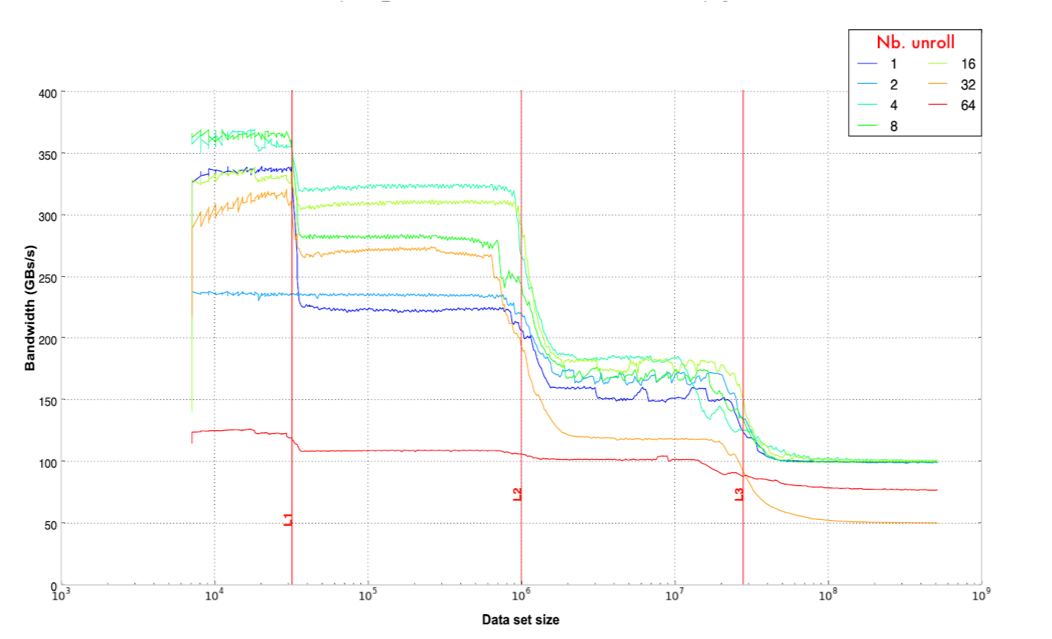
\includegraphics[width=16cm]{images/dml_unroll_best.png}
    \caption{\label{pic:dml_unroll_best} Performance de plusieurs déroulements pour une stride de 8 bytes (lecture de tous les éléments).}
    \end{figure}
    
    
    \subsubsection{Large page} \label{sec:dml_large_page}
    %%%%%%%%%%%%%%%%

    L'expérimentation suivante a pour objectif de comparer la performance du benchmark lors de l'utilisation de différentes tailles de pages mémoire. Comme présenté dans la \autoref{sec:page}, l'utilisation de page de plus grande taille permet d'améliorer la performance du système mémoire, notamment en accélérant le traitement de la TLB. Les pages plus larges permettent aussi de réduire les conflits d'associativité dans les caches. L'expérimentation réalisée avec un coeur actif a permis d'obtenir les résultats présentés dans le \autoref{tab:large_page_memory}. La performance des caches est améliorée avec l'utilisation des pages larges, jusqu'à 30\% dans le cache L3. Lorsque le jeu de donnée est dans le L3, la mesure du nombre d'évènements \textit{miss} de la TLB augmente d'un facteur 300. Cependant, la TLB arrive à masquer la majorité de ces \textit{miss} et conserve une bonne performance (150 GB/s).

    \begin{table}[]
    \centering
    \resizebox{\textwidth}{!}{%
    \begin{tabular}{l|c|c|c|c|c|}
    \cline{2-6}
     & \cellcolor[HTML]{EFEFEF}L1 (GB/s) & \cellcolor[HTML]{EFEFEF}L2 (GB/s) & \cellcolor[HTML]{EFEFEF}L3 (GB/s) & \cellcolor[HTML]{EFEFEF}Memoire (GB/s) & \cellcolor[HTML]{EFEFEF}dTLB-load-misses \\ \hline
    \multicolumn{1}{|l|}{\cellcolor[HTML]{EFEFEF}Page de 4 KiB} & 320 & 220 & 150 & 13.40 & 2254025 \\ \hline
    \multicolumn{1}{|l|}{\cellcolor[HTML]{EFEFEF}Page de 2 MiB} & 340 & 225 & 200 & 13.45 & 6556 \\ \hline
    \end{tabular}%
    }
    \caption{Performance du benchmark \texttt{DML\_MEM} utilisant deux tailles de pages. La performance dans les 4 niveaux de la hiérarchie mémoire a été mesurée avec le benchmark et le nombre d'évènements \textit{miss} lorsque le jeu de donnée est dans le cache L3.}
    \label{tab:large_page_memory}
    \end{table}
    
    
    Nous nous sommes ensuite intéressés aux performances du benchmark lorsque plusieurs coeurs sont actifs, avec et sans l'utilisation des pages larges. Nous observons les mêmes écarts de performances lorsque le jeu de données est stocké dans les caches. Lors de l'utilisation de pages standards (4 KiB), nous constatons que lorsque la taille du jeu de données approche de la taille des jeux de données, la performance commence à se détériorer. Avec l'utilisation des pages de 4 MiB, la performance dans chaque niveau de cache est constante et ne se détériore que lorsque le jeu de donnée dépasse la taille du niveau de cache. Cet effet observé lors de l'utilisation de petites pages est appelé \textit{page coloring} \cite{Zhang2009}.
  
    \begin{figure}
    \center
    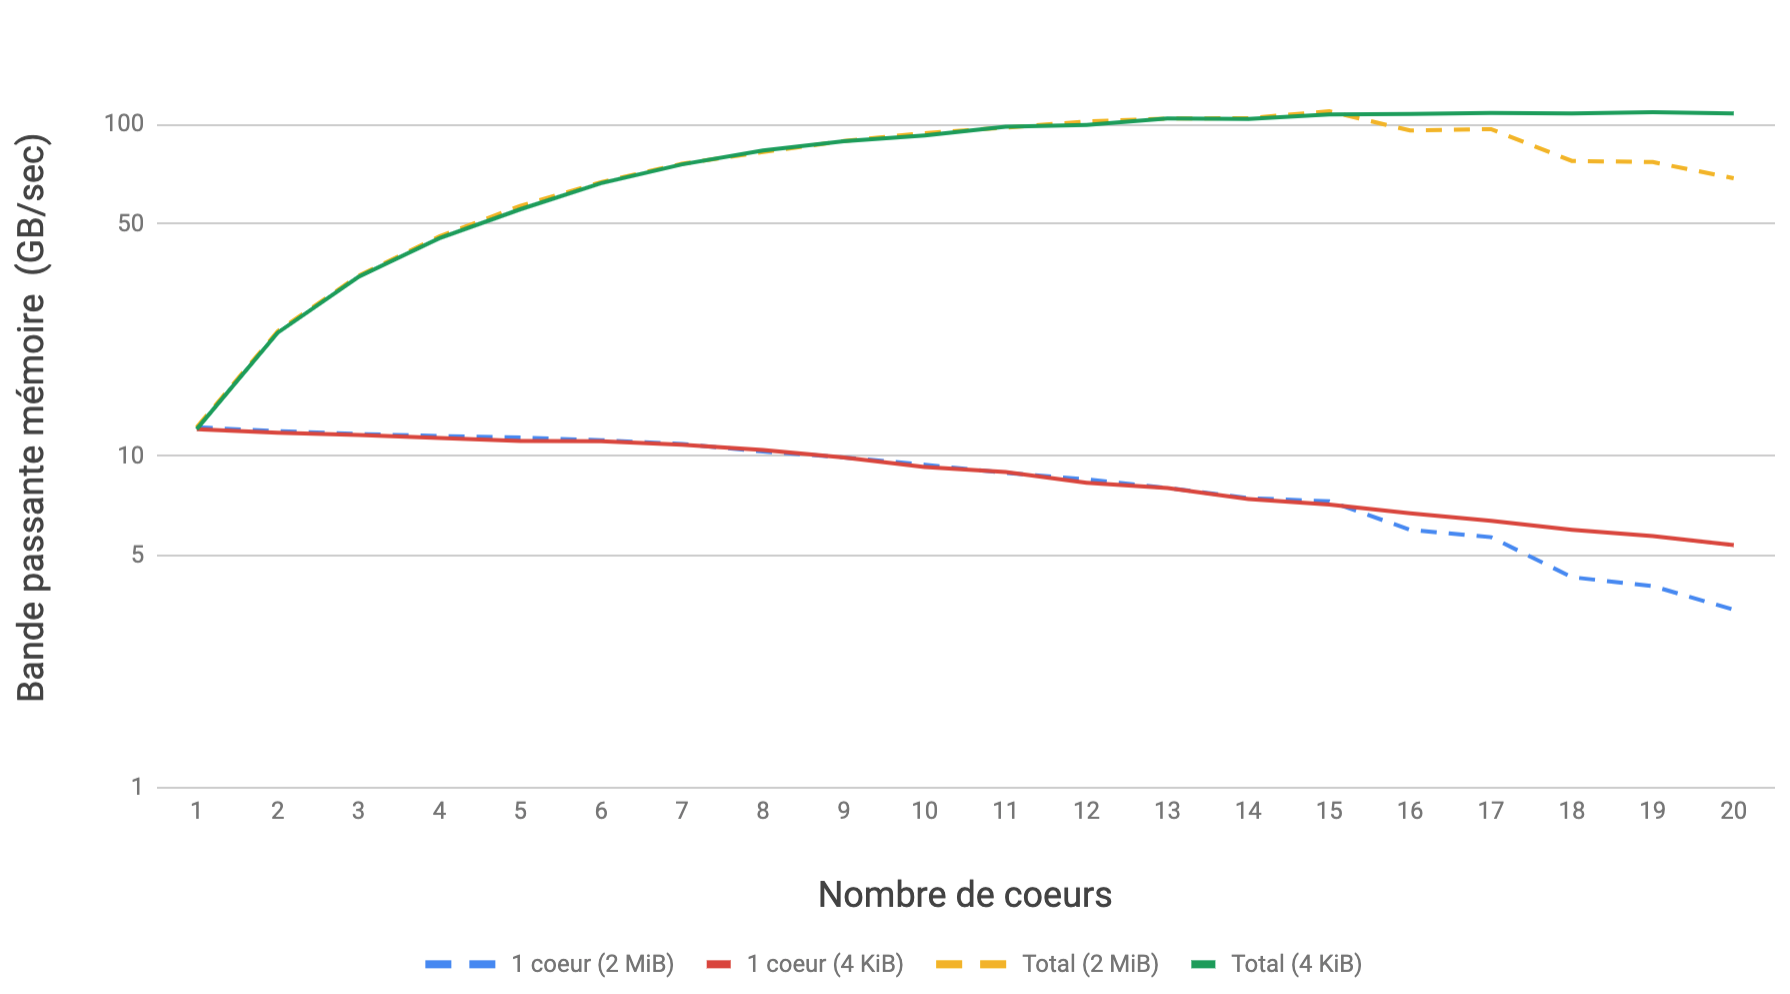
\includegraphics[width=14cm]{images/dml_large_page_bw.png}
    \caption{\label{pic:dml_large_page_bw} Bande passante mémoire par coeur et pour plusieurs coeurs utilisant deux tailles de pages pour stocker un jeu de données de 2 GiB.}
    \end{figure}
    
    Le graphique de la \autoref{pic:dml_large_page_bw} montre les performances du benchmark avec un ou plusieurs coeurs actifs sur un jeu de donnée de 2 GiB. Nous remarquons que la performance du benchmark baisse lorsqu’au moins 15 coeurs sont utilisés avec des pages larges. La performance par coeur diminue de 5.39 GB/s à 3.44 GB/s. Nous n'avons pour le moment pas réussi à expliquer ce problème qui affecte tous les jeux de données supérieurs à 2 GiB.
    
    Bien que la TLB limite rarement les performances des applications réelles, le recours à l'utilisation de pages larges peut être bénéfique. Les versions récentes du noyau Linux peuvent choisir elles-mêmes lors de l'allocation mémoire si le recours à des pages plus grandes peut être bénéfique pour l'application (Red Hat Transparent Huge Pages (THP)). Comme nous montrons dans cette dernière expérience que l'utilisation de page de 2 MiB peut détériorer les performances, il est conseillé que cette responsabilité revient à l'utilisateur qui devra décider ou non de leur utilisation en fonction de son application. 
  


    
    \subsubsection{Fréquence et coeurs: impact sur la bande passante} \label{sec:dml_core_vs_freq}
    %%%%%%%%%%%%%%%%
    
    Dans cette expérimentation nous avons mesuré la bande passante mémoire atteignable par notre benchmark pour différente configuration de fréquence et nombre de coeurs actifs. Les résultats sont visibles sur la \autoref{pic:dml_core_vs_freq}. Comme dans l'expérimentation précédente (\autoref{sec:dml_saturation}), nous démontrons que la totalité des coeurs n'est pas nécessaire pour saturer la bande passante. Cette expérience montre aussi que les coeurs utilisés n'ont pas besoin d'utiliser leur fréquence maximale. En effet, notre benchmark sature le bus mémoire avec 17 coeurs cadencés à seulement 2.1 GHz. Le script utilisé pour générer la \autoref{pic:dml_core_vs_freq} annote automatique le graphique pour identifier rapidement les maximums. Une telle utilisation du benchmark \verb=DML_MEM= permet d'identifier le couple  \verb|{fréquence, nombre de coeurs}| minimal pour saturer le bus mémoire. Pour des applications limitées par la performance de ce dernier, il peut être intéressant de désactiver les coeurs supplémentaires ou de plafonner la fréquence du processeur pour limiter la consommation électrique. En plus de vérifier la présence potentielle de bogues dans l'architecture, cette expérimentation peut permettre à un utilisateur de choisir la meilleure configuration pour un achat de nouveaux processeurs. 
    
    \begin{figure}
    \center
    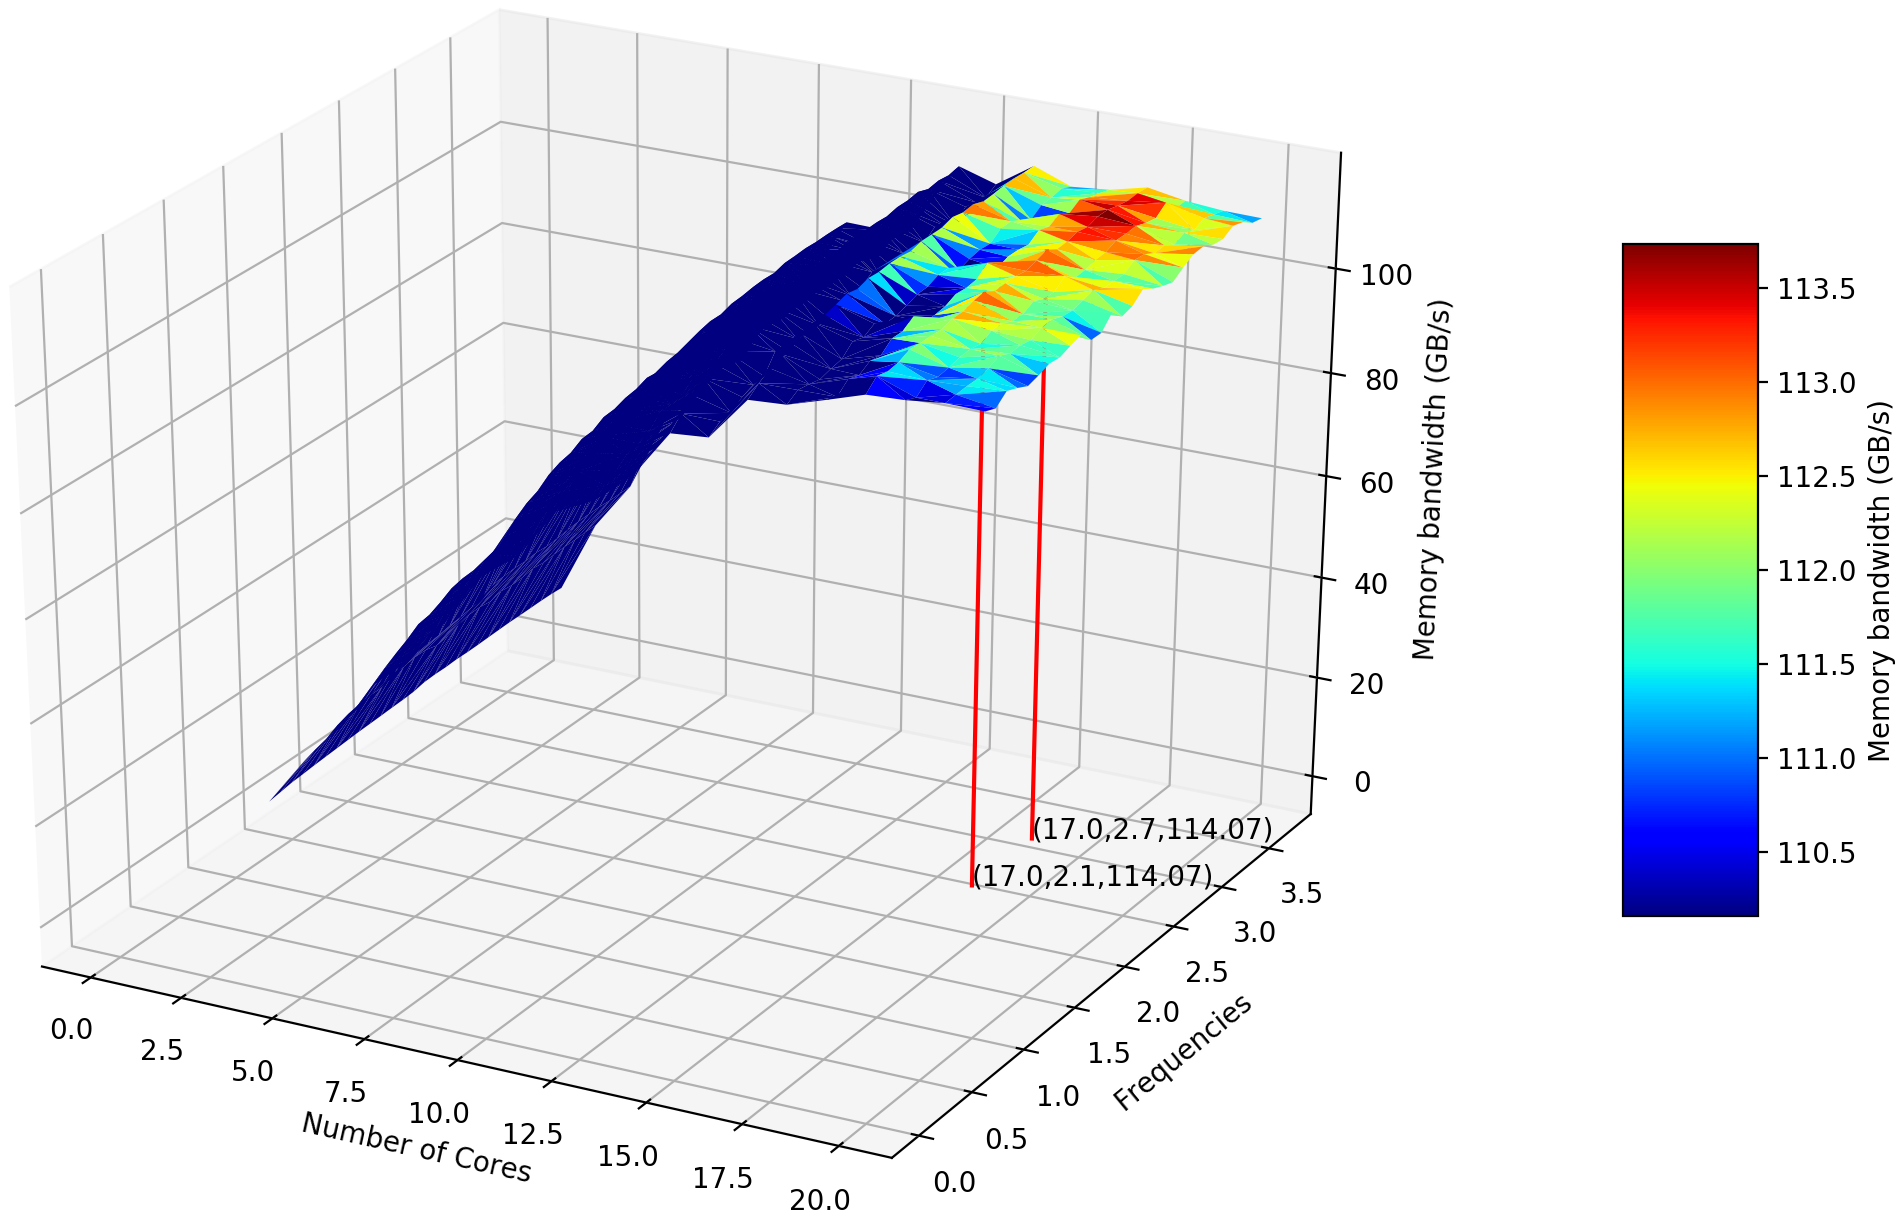
\includegraphics[width=14cm]{images/dml_core_vs_freq.png}
    \caption{\label{pic:dml_core_vs_freq} Mesure de la performance du bus mémoire lors de l'utilisation de différent nombre de coeurs plafonnés à différentes fréquences}
    \end{figure}
    


    
    

\subsection{Conclusion}
%%%%%%%%%%%%%%%%%%%%%%%%%%%%%%%%%%%%%%%%%%%%%%%%%%%%%%

    Cette section s'intéresse au \verb=DML_MEM=, un benchmark permettant de caractériser de multiples parties du système mémoire. Le benchmark permet de réaliser des accès mémoire grâce à des motifs de strides pour caractériser les plateformes pour des codes de types \textit{stencil}.
    Nous montrons que la microarchitecture peut avoir des comportements très inattendus lors de l'utilisation de certaines tailles de saut. À travers ces expérimentations nous souhaitons attirer l'attention du programmeur sur la complexité de la microarchitecture et de la nécessité de sa caractérisation.
    Lors des travaux de thèse, l'utilisation de cet outil nous a permis de caractériser plusieurs plateformes différentes et de déceler des bugs majeurs dans certaines d'entre elles. Les accès par stride mettent la pression sur le pré-chargeur mémoire, l'utilisation de cet outil peut alors être aussi intéressante lors de la conception d'une nouvelle architecture que lors de sa caractérisation pour le portable d'une application réelle. 